\sys exposes non-volatile memory for \emph{protected} variables to
the application as a virtual address space partitioned into pages.
Paged virtual memory is a key enabler of task coalescing, which
we described in Section~\ref{sec:task_coalescing}. Virtualization simplifies
coalescing, because the system gets the freedom to move application's data
between volatile and non-volatile memory transparently.
%
\sys manages memory such that application tasks operate primarily from
efficient volatile SRAM rather than non-volatile FRAM, which is more costly to access than SRAM,
as we showed in Figure~\ref{fig:framEnergy}. \sys runtime implements memory
virtualization by moving pages of the address space from the large,
non-volatile memory to a small, volatile memory on demand and writing all dirty
pages back atomically. Since memory moves are at page granularity, \sys
exploits hardware\hyp{}accelerated block copies.

%\subsection{Paged Non-Volatile Virtual Memory} 

As they are
accessed by a task, pages are swapped from their home location
in the direct\hyp{}mapped non-volatile memory, called
\texttt{\underline{store}} (underline denotes allocation in non-volatile
memory) into the fully\hyp{}associative \texttt{working} page buffer in volatile memory. The
\texttt{working} buffer is allocated to take up the volatile memory that
remains after space for stack is allocated.
%
\sys uses two-phase commit to write dirty pages from the \texttt{working} buffer
back to their home location in \texttt{\underline{store}} atomically,
ensuring data consistency even with power failures.
%
When any dirty page is swapped out from the \texttt{working} buffer due to
eviction or task transition from last coalesced task, the first phase writes
the page to a direct\hyp{}mapped non-volatile \texttt{\underline{shadow}}
buffer, and the second phase writes it from
\texttt{\underline{shadow}} to \texttt{\underline{store}}.
%
Unlike prior work~\cite{chain,alpaca} that moves scattered variables one at a
time between volatile and non-volatile memory, \sys's page-based
design moves contiguous blocks of data.
%
\sys takes full advantage of hardware\hyp{}accelerated block copies using
Direct Memory Access (DMA) hardware in common microcontrollers --- e.g. 5x
fewer cycles on MSP430FRxxxx.

\subsection{Address Translation and Variable Access}

A \sys task must access protected non-volatile variables through a restricted memory
interface. The interface includes \texttt{RVAR(var)}, which reads the value of
variable {\tt var} and \texttt{WVAR} \texttt{(var,val)}, which assigns
value {\tt val} to variable {\tt var}. The implementation of {\tt
RVAR} is shown in Algorithm~\ref{algo:rwar} and {\tt WVAR} implementation is
similar except for an assignment instead of the return.
%
{\tt RVAR} and {\tt WVAR} operations translate a variable's physical address in non-volatile memory into a \emph{virtual address} in the page buffer in volatile memory.  In \sys, a virtual address is composed of a \emph{page tag} that identifies the page and a \emph{page offset} that identifies a byte.

%How an $a$-bit memory address decomposes into a tag and an offset depends on the number (and size) of each page of protected memory. To address {\tt p} pages of size {\tt s}, a tag comprises $log(p)$ bits, the offset comprises $log(s)$ bits and $log(p) + log(s) = a$. For example, in a 16-bit address space (i.e., 16\,kB of protected memory) with 512 pages of 128 bytes each, a page's tag is the high-order nine bits of the address and a byte's page offset is the remaining 7 bits.

\begin{algorithm}[t]
	\caption{\texttt{RVAR}(variable $v$)}
	\label{algo:rwar}
	\scriptsize
	%\small
	\begin{algorithmic}[1]
		\State $t \leftarrow \Call{GetTag}{v}$ 
        \State $i \gets \{ j\ |\ \Call{GetTag}{\texttt{working}[j]} = t \}$ \Comment{Look in the page buffer}
		\If { $i = \emptyset$ } \Comment{Is the variable in a resident page?}
		\State	$i \gets \Call{PageFault}{t}$ \Comment{Page in from non-volatile memory}
		\EndIf
		\State $o \leftarrow \Call{GetOffset}{v}$ 		
		\State \Return \texttt{working}[$i$][$o$]  \Comment{Return directly from page buffer}
	\end{algorithmic}
\end{algorithm}

After address translation, \sys attempts to access the protected variable's
location in the volatile paging buffer. \sys keeps track of the page tags for
the pages currently resident in the paging buffer. When a task accesses a
variable, it compares the variable's page tag to tags of the pages in {\tt
working} (Line 2).
%
%If the accessed variable's page is resident in the page buffer,
%then the tag of one of the pages in this buffer is equal to the accessed
%variable's page tag.
%
If the accessed variable's page tag is not found in the page buffer, the
operation incurs a {\em page fault} (Line 4). At a page fault, \sys must swap
out one of the pages that is resident in the page buffer (to the non-volatile
commit buffer, \texttt{\underline{shadow}}) and swap in the variable's page.
%
The byte is accessed in the page buffer at the index of the resident page and
the variable's page offset (Lines 5-6).

%Algorithm~\ref{algo:rwar} shows pseudo-code of \texttt{RVAR} and we omit a listing for {\tt WVAR} as it is very similar except it writes the memory location and returns nothing. If the page tag of the variable \texttt{var} is not found in \texttt{working} (e.g. Lines 2--3), there is a page fault that requires a new page to be swapped in to the page buffer.

\subsection{Page Faults and Page Swapping}

\begin{algorithm}
	\caption{\texttt{PageFault}(tag $t$)}
	\label{algo:pagefault}
	\scriptsize
	%\small
	\begin{algorithmic}[1]
        \State \LeftComment{$i_\text{victim}$: volatile index to next free slot or page to be evicted, set to 0 at boot}
        \State \LeftComment{\texttt{\underline{numShadowed}}: non-volatile, reset to 0 on boot unless in phase 2 commit}
        \State $t_\text{victim} \gets \Call{Tag}{\texttt{working}[i_\text{victim}]}$
		\If {\Call{IsDirty}{working[$i_\text{victim}$]} }	\Comment{Are we evicting a dirty page?}
		\State $\texttt{\underline{shadow}}[t_\text{victim}] \xleftarrow{\text{DMA}} \texttt{working}[i_\text{victim}]$
            \Comment{Swap out the page}
        \If {$t_\text{victim} \not\in \texttt{\underline{shadowList}}$} \Comment{Keep track as list for quick traversal}
            \State $\texttt{\underline{shadowList}}[\texttt{numShadowed++}] \gets t_\text{victim}$
        \EndIf
		\EndIf
		\If {\Call{IsValid}{\underline{shadow}[$t$]}} \Comment{Had the page been swapped out earlier?}
		\State $\texttt{working}[i_\text{victim}] \xleftarrow{\text{DMA}} \texttt{\underline{shadow}}[t]$
            \Comment{Get page from commit buffer}
		\Else
		\State $\texttt{working}[i_\text{victim}] \xleftarrow{\text{DMA}} \texttt{\underline{store}}[t]$
            \Comment{Get page from backing store}
		\EndIf 
        \State $i_\text{victim} \gets (i_\text{victim} + 1) \mod |\texttt{pageBuf}|$ \Comment{FIFO eviction policy}
	\end{algorithmic}
\end{algorithm}

A page fault on a memory access requires \sys to swap out one of the pages in
the page buffer, i.e. \emph{victim page}, preserving updates made to that page,
and to copy the accessed page of protected data into the page buffer.
Algorithm~\ref{algo:pagefault} shows how \sys handles a page fault. A victim
page in the \texttt{working} buffer is selected for eviction according to
\emph{first-in-first-out} replacement policy (Lines 2 and 12).  If the page
being swapped out is not dirty and the page being accessed had not been dirtied
and swapped out to the \texttt{shadow} buffer since last boot, then
handling a page fault consists of copying the accessed page from
\texttt{\underline{store}} into the \texttt{working} buffer (Line 11).
Otherwise, the page fault handler must take the following extra steps.

If a task modified any byte in the victim page
(i.e.,  using \texttt{WVAR}), then the page is dirty. Before swapping in the
accessed page, \sys must first preserve the updated values in the dirty page so
that they can be committed back to their locations in memory
when the dynamic task ends (but not earlier). To preserve dirty values, \sys
copies the victim page to the non-volatile \texttt{\underline{shadow}}
buffer (Line 5) and records the page's tag in a non-volatile list (Lines 6-7)
to support iteration over shadow pages having traversing all slots in the
buffer, necessary in the second phase of the commit.
%
%Dirty pages remain in {\tt \underline{shadow}} buffer until the
%dynamic task completes, at which point \sys commits the modified
%pages from {\tt \underline{shadow}} back to \texttt{\underline{store}}.
%
If the accessed page was previously modified and
swapped out since the last boot (Line 8), the most recent contents of the page is in {\tt
\underline{shadow}}, not \texttt{\underline{store}} (Line 9).

%As
%Algorithm~\ref{algo:pagefault} shows in Line 4, \sys checks if the requested
%page was previously modified by the executing task. To track whether a page is
%modified, \sys stores a dirty bit with the page and sets it when the page is
%written to. If an accessed page's dirty bit is set, the page must be swapped in
%from \texttt{\underline{shadow}} rather than its original memory location (Line 5),
%furnishing the task with the page's modified values. If the accessed page is
%not dirty, \sys swaps it in from its original location in memory (Line 7).

%
%\sys
%uses DMA block copies for all page swapping operations, leveraging the
%efficiency of hardware support.

\subsection{Atomic Two-Phase Commit of Dirty Pages}

When the last task in a coalesced group completes, \sys must commit \emph{all}
dirty pages in the \texttt{working} buffer and the swapped out pages in
\texttt{\underline{shadow}} buffer back to their original locations in
\texttt{\underline{store}}. If a task is allowed to (re-)execute after only
\emph{some} pages have been copied to \texttt{\underline{store}}, that task
might see protected variables in an inconsistent state.

To make the commit atomic, \sys copies the pages in two phases, implemented by
Algorithm~\ref{algo:commit}.
%
The first phase copies dirty pages in \texttt{working}
buffer to the non-volatile \texttt{\underline{shadow}} buffer (Line 4). 
The second phase, copies pages from \texttt{\underline{shadow}} to \texttt{store} (Line 12).
If power fails during the first phase, the whole
commit is aborted, and the dynamic coalesced task restarts from its first
static task. If power fails in the second phase, the commit will be safely
resumed on next boot.
The non-volatile metadata for the second phase is the \texttt{\underline{committing}}
bit, which is set before the first page is copied (Line 9) and cleared after the last
page is copied (Line 14), and \texttt{\underline{numShadowed}} counter, which
indexes into the \texttt{\underline{shadowList}} (Line 11), is
decremented after each page is copied (Line 13), and cleared once the phase
completes (Line 18).

\sys non-volatile \texttt{\underline{shadowList/numShadowed}} implementation is
a more efficient alternative to a simpler implementation that keeps a valid bit
in each entry of \texttt{\underline{shadow}} and, on every boot into second
phase, traverses all entries, copying the pages with a set bit, and
clearing the bit.
%
\sys assumes that the write to a non-volatile word in memory is atomic.

\begin{algorithm}[t]
	\caption{Two-phase commit}
	\label{algo:commit}
	\scriptsize
	%\small
	\begin{algorithmic}[1]
        \Procedure{CommitPhase1}{} \Comment{Invoked from \texttt{next\_task} on last coalesced task}
            \For {$i \in 0..|\texttt{working}|-1$}
                \State $t \gets \Call{Tag}{\texttt{working}[i]}$
                \State $\texttt{\underline{shadow}}[\Call{Tag}{\texttt{working}[i]}] \xleftarrow{\text{DMA}} \texttt{working}[i]$
                \State $\texttt{\underline{shadowList}}[\texttt{\underline{numShadowed}}] \gets t$
                \State $\texttt{\underline{numShadowed}} \gets \texttt{\underline{numShadowed}} + 1$
            \EndFor
            \State \Call{CommitPhase2}{}
        \EndProcedure
        \Procedure{CommitPhase2}{}
            \State $\texttt{\underline{committing}} \gets \textbf{true}$
            \While{\texttt{\underline{numShadowed}} > 0}
                \State $t \gets \texttt{\underline{shadowList}}[\texttt{\underline{numShadowed}} - 1]$
                \State $\texttt{\underline{store}}[t] \xleftarrow{\text{DMA}} \texttt{\underline{shadow}}[t]$
                \State $\texttt{\underline{shadow}}[t] \gets \textbf{nil}$ \Comment{Clear entry for page fault handler}
                \State $\texttt{\underline{numShadowed}} \gets \texttt{\underline{numShadowed}} - 1 $
            \EndWhile
            \State $\texttt{\underline{committing}} \gets \textbf{false}$
        \EndProcedure
        \Procedure{OnBoot}{} \Comment{Invoked on every boot, before transitioning to a task}
            \If { \texttt{\underline{committing}} } \Call{CommitPhase2}{}
            \EndIf 
            \State $\texttt{\underline{numShadowed}} \gets 0$, $i_\text{victim} \gets 0$
        \EndProcedure
	\end{algorithmic}
\end{algorithm}

%\subsection{Paging Example}
%
%Figure~\ref{fig:volatile-buffer} illustrates the execution of a simple task using \sys's paging mechanism. The task manipulates the protected variables {\tt x}, {\tt y}, and {\tt z}. The variables {\tt y} and {\tt z} are in the same page and they are currently in the volatile page buffer---on accessing {\tt y} and {\tt z}, the task needs only to access \texttt{pageBuf}. Since variable \texttt{x} is kept in a different page in \texttt{pagesOrg}, accessing it creates a page fault. At this point, \sys swaps the active page in \texttt{working} by committing it into the non-volatile {\tt \underline{shadow}} region and copying the corresponding page from \texttt{pagesOrg} to \texttt{pageBuf}. When the task completes, \sys sets the commit bit, copies the dirty page from \texttt{pagesTmp} to its original location in \texttt{pagesOrg} and unsets the commit bit.

%\begin{figure}[t]
%	\centering
%	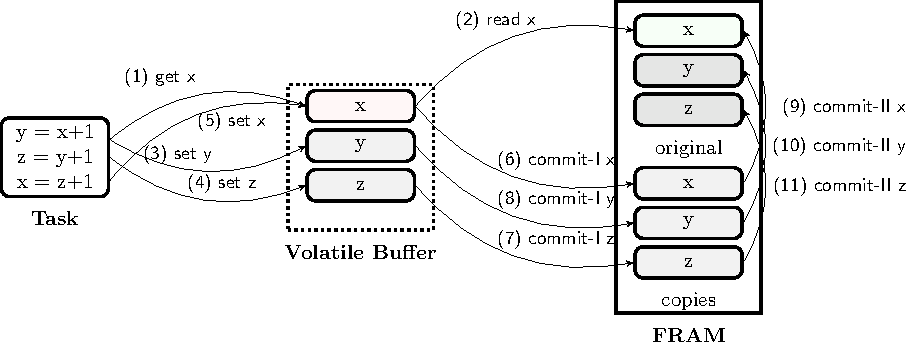
\includegraphics[width=0.75\columnwidth]{figures/sram-buffer}
%	\caption{The interaction between the task, volatile buffer and the non-volatile memory (FRAM). Initially, the persistent variable \texttt{x} is not in the volatile buffer but \texttt{y} and \texttt{z} are.}
%	\label{fig:volatile-buffer}
%\end{figure}

%\subsection{Memory Consistency}

\textbf{Memory Consistency.} \sys's paging mechanism ensures that a task only ever executes using consistent
protected data. During task execution, modifications to protected data do not
affect their original memory locations, because a task reads and writes the
volatile \texttt{working} buffer only, and modified pages are kept in
\texttt{\underline{shadow}} until commit. A power failure erases the contents
of the page buffer, preventing a re-executing task from observing updates in
the page buffer from a previous execution attempt. Clearing \texttt{\underline{shadow}}
entries as part of the second phase commit (Line 13), ensures that all accesses to
protected variables in subsequent tasks correctly access their original memory
locations in \texttt{\underline{store}}.
%
%The non-volatile commit bit persists
%across power failures and \sys repeatedly attempts to commit until it succeeds,
%despite arbitrary power failures.

%\subsection{Managing Paging Overhead}
%
%The efficiency of \sys's paging scheme relies on the fact that data in pages are contiguous, which makes them amenable to being manipulated by hardware assisted DMA bulk copy operations. To justify this design choice we experimentally evaluated the efficiency of using DMA block copies, compared to explicit, software copy loops. We copied blocks of data of different size between memory regions on a WISP~\cite{wisp} using a hand-written loop and using DMA (refer to Section~\ref{sec:results_hardware} for hardware setup details). Figure~\ref{fig:dmaTimeEnergy} shows that for moving large blocks of data like a page, hardware DMA is considerably better than software in both run time and energy efficiency. \sys's design moves data in pages, not individual words, leveraging the increased efficiency of DMA data movement.
%
%\begin{figure}[t]
%	\centering
%	\subfloat[Time needed to transfer a block of data]{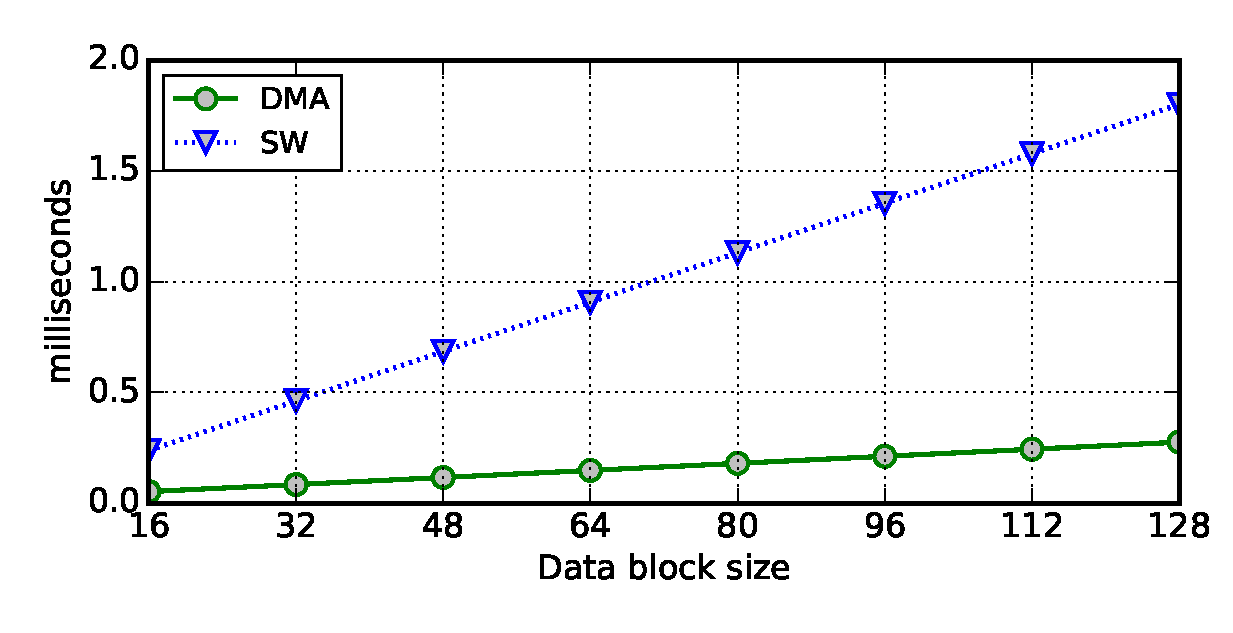
\includegraphics[width=0.49\columnwidth]{figures/dmaSize_time.eps} }
%	\subfloat[Energy needed to transfer a block of data]{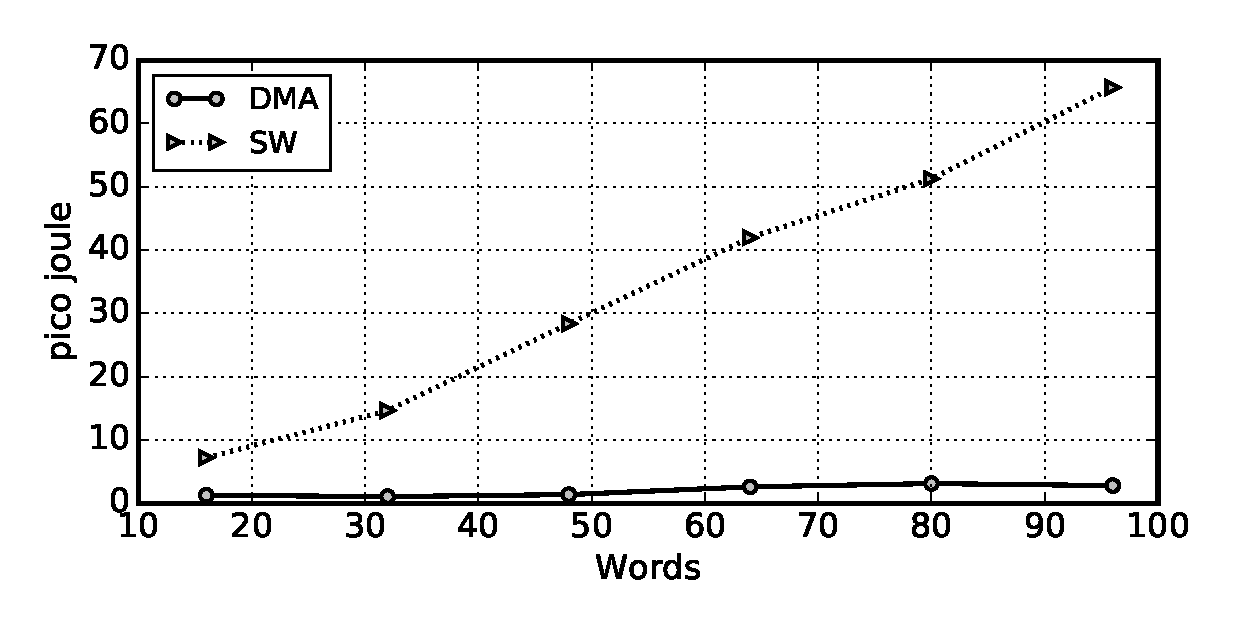
\includegraphics[width=0.49\columnwidth]{figures/energyConsumptionDMA_SW.eps}}
%	\caption{Time and energy consumption of moving a block of data from SRAM to FRAM: CPU intervention versus Direct Memory Access (DMA).\todo{Explain HW/SW setup; make fonts larger, unify legends and axes}{Amjad}}
%	\label{fig:dmaTimeEnergy}
%\end{figure}
